\documentclass[times, 10pt]{thesisMDH}
\addbibresource{references.bib}

% --- Pacages -----
\usepackage[ddmmyyyy]{datetime}
\usepackage{graphicx}
% \usepackage{epsfig} % Used to load plantuml
\usepackage{epstopdf} %converting to PDF
% \usepackage{amsmath} % Dep mathtools
\usepackage{amsfonts} % dep
\usepackage[utf8]{inputenc}
%% Maths
\usepackage{mathtools} % Loads asmath
\usepackage{fancyhdr}
\usepackage{xparse} % Used to provide \NewDocumentCommand.
\usepackage{enumerate}
\usepackage{pdflscape}
% \usepackage{listings}     % Do not list codes in paper use bellow.
% \usepackage{algpseudocode} % Algorithms instead of listings
\usepackage[noend]{algpseudocode}
%\usepackage{algorithm,algorithmic}
\usepackage{algorithm}
% \usepackage{ragged2e}
\usepackage[document]{ragged2e}
% \usepackage[linesnumbered,vlined,ruled,scleft]{algorithm2e}
% \usepackage[titletoc]{appendix}

\usepackage[margin=3cm]{geometry}
\usepackage[absolute]{textpos}
\usepackage[section]{placeins}
\usepackage{url}
\usepackage{tabularx}
\usepackage{acronym}
\usepackage{harpoon}  % Long vector arrows. perhaps DEP
\usepackage{gensymb}
\usepackage{caption}
\usepackage{subcaption}
\usepackage{todonotes}
\usepackage{multirow}
\usepackage{titlesec}

\usepackage{cprotect} % Use verb in figure captions

% Bibliography settings:

% \titleformat{\subsection}
% {\normalfont\small% Changed!
%   \bfseries}{\thesection}{1em}{}[{\titlerule[0.8pt]}]

\graphicspath{{Figures/}{figures/}{.}{images/}{results/}} %Setting the graphicspath

%%%%%%% Import tikz for a figure.
\usepackage{tikz}
% \usepackage{plantuml}
\usepackage{ifluatex}
% \ifluatex
%     \usepackage{pdftexcmds} %
%     \makeatletter%
%     \let\pdfstrcmp\pdf@strcmp%
%     \let\pdffilemoddate\pdf@filemoddate%
%     \makeatother%
% \fi
\usepackage[clean]{svg}
% \usepackage{svg}
\svgpath{figures}

\usetikzlibrary{automata, positioning, arrows}
\tikzset{
    ->, % makes the edges directed
    >=stealth,
    %>=stealth’, % makes the arrow heads bold
    node distance=3cm, % specifies the minimum distance between two nodes. Change if necessary.
    every state/.style={thick, fill=gray!10}, % sets the properties for each ’state’ node
    initial text=$ $, % sets the text that appears on the start arrow
}
\tikzset{aruco/.style={
        rectangle, draw=black!50, fill=black!20, thick, minimum width=0.85cm, minimum height = 0.85cm,
    }
}
%%%%%%%% ----------------
%% =========={ Commando creation }==========
% \renewcommand\thesection{\arabic{section}}
% \newcommand{\lit}[1]{\item[\textbf{L#1}]
%\newcommand\req[1]{%
%    \item["\textbf{RQ#1}"]%
%    }%
% \newcommand\req[1]{\item[\textbf{RQ#1}]}
% \newcommand{\rew}[1]{{\color{red}#1}
% \newcommand{\rewc}[2]{{\color{#2}#1}
%\newcommand{\rewdetail}[2]{{\color{red}#1\todo[color=red!40]{#2}}
%\newcommand{\insertref}[1]{\todo[color=green!40]{#1}
%%\newcommand{\explainindetail}[1]{\todo[color=red!40]{#1}}
%\newcommand{\setseparation}{\setlength\itemsep{0mm}
%\def\checkmark{\tikz\fill[scale=0.6](0,.35) -- (.25,0) -- (1,.7) -- (.25,.15) -- cycle;}
%\newcommand{\cspace}{\ensuremath{\mathcal{C}}


% \renewcommand{\headrulewidth}{0.4pt}
% \renewcommand{\footrulewidth}{0.4pt}
% \newcommand\node[2]{%
% \item[%
% \textbf{#1}%
% ] \textbf{#2}%
% }

% % \newcommand{\R}{\(\mathbb{R}\)}
% \newcommand*\aruco[1]{ArUco#1}
\NewDocumentCommand\aruco{}{
    \IfNoValueTF{#1}
        Aruco
        Aruco#1}
\newcommand*\arucoS{\aruco{ }}
\NewDocumentCommand\openpose{}{OpenPose }
% {\IfNoValueTF{#1}{No open}{OpenPose#1}}
\newcommand*\openposeS{\openpose{ }}
\newcommand*\Q[1]{$Q_#1$}
\newcommand*\R{\mathbb{R}}
\newcommand*\defref[1]{Definition~\ref{#1}}
% \newcommand*\NN{\mathbb{N}} % natural numbers
\newcommand*\NN{\mathbb{N}} % natural numbers
\newcommand*\AAA{\mathcal{A}} % automaton
\newcommand*\WWW{\mathring{W}^2_1} % Sobolev space 2,1,o
\newcommand*\defined[1]{\emph{#1}} % used for defining new terms
\DeclarePairedDelimiter\abs{\lvert}{\rvert} % proper absolute value

% Larger \mu and \sigma for hypothesis question
\NewDocumentCommand\bigmu{}{%
    \makebox{%
        \Large\ensuremath{\mu}
    }%
}%
\NewDocumentCommand\bigsigma{}{%
    \makebox{%
        \Large\ensuremath{\sigma}%
    }%
}%
% \newcommand{\bigmu}{\raisebox{-.20\baselineskip}{\ensuremath{\mu}}}
% \newcommand{\bigsigma}{\raisebox{-.20\baselineskip}{\ensuremath{\sigma}}}

% \newcommand{\annoterel}[2]{%
%   \overset{%
%     \substack{\hidewidth\text{#1}\hidewidth\\\downarrow}%
%   }{#2}%
% }
\NewDocumentCommand\annoterel{mm}{%
  \overset{%
    \substack{\hidewidth\text{#1}\hidewidth\\\downarrow}%
  }{#2}%
}


\usepackage[pdfborder={0 0 0},colorlinks=true,urlcolor=blue,citecolor=red,bookmarks=false]{hyperref}


%%%%% Title page settings
\fancyHeader{Valid OpenPose on laying humans}{Magnus Sörensen}
\university{Mälardalen University}
\department{School of Innovation Design and Engineering\\ Västerås, Sweden}
\subject{Thesis for the Degree of Master of Science in Engineering - Robotics 30.0 credits}
\thesisTitle{Validation of OpenPose on laying humans using statistics, Aruco corners and a novel minimal point of error}
\authorOne{Magnus Sörensen}{msn15018@student.mdh.se}
%\authorTwo{Student Name2}{studentEmail@student.mdh.se}


\examiner{Martin Ekstr\"{o}m}{M\"{o}lardalen University, V\"{ä}sterås, Sweden}
\supervisorA{Fredrik Ekstrand}{M\"{a}lardalen University, V\"{a}sterås, Sweden}
\supervisorB{Joaqu in Ballestero}
{University of M\'{a}laga, M\'{a}laga, Spain}
\supervisorC{Jesus Manuel Gomez de Gabriel Ballesteros}{University of M\'{a}laga, M\'{a}laga, Spain}

\theDate{\today}
%%%%% END

\begin{document}
\titlePage
% Begin actual text
\frontmatter
%\input{sections/000-guideline} % Remove 000-guideline section
\input{sections/abstract}
\newpage
%%========= Tables ==========
{\hypersetup{linkcolor=black}\tableofcontents}
\clearpage
{\hypersetup{linkcolor=black}\listoffigures}
\clearpage
{\hypersetup{linkcolor=black}\listoftables}

\mainmatter
\section*{Acronyms}
\begin{acronym}[MPC] % Give the longest label here so that the list is nicely aligned
    %\acro{MPC}{model predictive control}
    %\acro{ros}[ROS]{Robot Operating System}
    %\acro{2d}[2D]{two-dimensional}
  %  \acro{3d}[3D]{three-dimensional}
    %\acro{dof}[DOF]{Degrees Of Freedom}
    \acro{uma}[UMA]{University of Malaga}
    \acro{mdh}[MDH]{University of Märlardalen}
    %\acro{ompl}[OMPL]{Open Motion Planning Library}
    %\acro{stomp}[STOMP]{Stochastic Trajectory Optimization for Motion Planning}
    %\acro{rrt}[RRT]{Rapidly exploring Random Tree}
    %\acro{t-rrt}[T-RRT]{Transitionbased Rapidly exploring Random Tree}
    \acro{cnn}[CNN]{Convolutional Neural Network}
    %\acro{gnn}[GNN]{Generative Neural Network}
    %\acro{rpm}[RPM]{Relative Position Map}  % <- fix this one
    %\acro{spars}[SPARS]{SPArse Roadmap Spanners}
    %\acro{hri}[HRI]{Human Robot Interaction}
    %\acro{phri}[pHRI]{Physical Human Robot Interaction}
    % \acro{cum}[CUM]{Camera Utility Mechanism}
    %\acro{cum}[RCPA]{Radial Camera Position Armature}
    %\acro{}[RPi]{Raspberry Pi}
    \acro{ar}[AR]{Augmented Reality}
    \acro{slp}[SLP]{Simultaneously-collected multimodal Lying Pose}
    \acro{rgb}[RGB]{RGB color space}
    \acro{rgbd}[RGBD]{RGB color space with depth}
    \acro{lwir}[LWIR]{Long-wave infrared}
    \acro{slam}[SLAM]{Simultaneous Localization and Mapping}
    \acro{vslam}[VSLAM]{Visual Simultaneous Localization and Mapping}
    \acro{vr}[VR]{Virtual reality}
    \acro{sfm}[SfM]{Structure from Motion}
    \acro{csv}[CSV]{Comma Separated Values}
    \acro{api}[API]{Application Programming Interface}
    \acro{imu}[IMU]{inertial measurement unit}
    \acro{uav}[UAV]{Unmanned aerial vehicle}
    \acro{uml}[UML]{Unified Modeling Language}
    \acro{iot}[IoT]{Internet of Things}
    % \acro{}[]{}
    % \acro{}[]{}
    % \acro{}[]{}
    % \acro{}[]{}
    % \acro{}[]{}
    % \acro{}[]{}
    % \acro{}[]{}
\end{acronym}

\newpage
% ===== Content: Modify the structure according to your needs =======
\section{Introduction}%
\label{sec:intro}
The motivation for this report the constant aging population in the western and eaten world.
This aging going up is a sign that the world are a bit more piece full, with out any major wars, hunger and general destruction.
According to OECD~\cite{oecd2018oecd}, the elderly population in Europe is about 20\% of population and Japan is on 27\%.
The increasing elderly population requires an increasing part of the younger population to take care of the elderly.
This could led to a downward spiral where as the numerous elderly increases more and more resources is needed to maintain a good living standard for the elderly, while less and less resources is created due to the younger generation is more and more occupied with taking care of the elders.

To counteract that future many companies is looking toward robotics and automations to find a solution.
Just searching for "Elderly" in a data base for technical research papers would give you over 7000 papers on the subject.
The authors Soren Tranberg et,al~\cite{Hansen2010evalrobot} also evaluated the use of robotics in healthcare already in 2010.
They conclude that the acceptance for robotics is high but considered that the products where unstable or complicated the concluding benefits was vague.

What drew the author to this subject is the challenging nature of creating such assist system.
Questions like how can that be done with out creating a system that are more expensive then a car.
Can sparse reconstruction really be done safely or is there any hidden limitations in the question it self.
But also soft questions like, would elderly trust the robot enough to dare to use it for its intended purpose?

The \ac{uma} is creating a robot that would have the task to to assist the elderly.
In this case the assist is to help an elderly subject on the flour to stand back up again with out calling for extra personal.
This is also not purl for economical reasons but also for a sens of self and a way to respect privacy of the subject.

% In their approach, they are set on using \openpose in a single camera configuration to find and assist the elderly.
\ac{uma}'s approach uses a robot arm with a single camera mounted on the gripper of the robot.
As this robot only have one camera mounted on the robot arm the 3D reconstruction of the subject needs to be completed by other methods then using binocular stereo vision as the robot in the paper~\cite{borangiu2010robot}.
One such solution is tho simply move the robot arm to two different position and the use same technique.
The draw back of that is the computational load for reconstructing the entire scene.
That is expensive and slow.

At \ac{uma} instead the approach is to use a preprocessing step to reduce the features in the image to a approximated skeleton of the subject.
Thus the expected outcome is to reduce several images in to its core components, the skeleton.
Then if each image contains its own skeleton the spars 3D reconstruction of the skeleton can be derived from those images.
However the above assumes that the camera position for each image is known and in this work that is not the case.
Instead this paper uses fiducial markers to identify the camera position for each image.

The question then is can a system that uses a single camera be used to do a sparse 3D reconstruction of the subject at hand and can that be done from all directions and angles?

The related works~\ref{sec:related_work} explore the \openpose algorithm for a way to do the sparse 2D reconstruction that later is used to do the space 3D reconstruction by using fiducial markers for the camera position is covered in Method~\ref{sec:method}.

% One such system that can be used to generate the skeleton of the subject is \opnpose algorithm.
% \openpose is a OpenSource product that uses part affinity fields with a \ac{cnn} to generate the skeleton from the subject in the image.
% To then reconstruction the sparse representation of the 3D skeleton using \openpose the intended system will use \aruco corners to determine the position of the camera in relation to the skeleton in the figure to generate the sparse 3D representation of the skeleton.

% This paper aims to answer if such system could be used to correctly classify the subjects limbs from all angles and what will happen if the spatial position derived by just using the input images.

% But in order to get an accurate description of the skeleton the input from the 2D skeleton needs to be sufficient.

% And the main problem with the approach of using \openpose is that it is trained on subjects that is standing, walking/running and sitting but the subjects in that \ac{uma} tries to assist are on the ground.
% This then is also covered by this report by using statistics on the results from the \openpose algorithm.










% Thus it is relevant to investigate how \openpose reacts if an elderly human is lying on the ground.
% robot is used to either assist or pick them up.
%In this thesis, an investigation to how OpenPose
% The problem is that OpenPose only seems to be trained on datasets where humans are standing, sitting, walking and running.

% Later, that was proven to be unsolvable due to a cumulative error when traversing the nodes.


% \subsection{Structure of this report}%
% \label{sub:Structure_of_this_report}
\textbf{Structure of the report}\\
The general structure of this document is as follows:
The Related Works in~\ref{sec:related_work} will discuss what others have done in this field of study.
Method~\ref{sec:method} derives the necessary steps and forms a hypothesis to solve the problem.
There is an ethics section~\ref{sec:ethics} that discusses the ethical part of this report and the licenses of the figures in the report.
Results~\ref{sec:results} show the results from the experiments and systems.
Discussion~\ref{sec:discussion} is the authors reflection on the results.
Conclusion~\ref{sec:conclusion} summarizes the findings of the report.
Appendices~\ref{sec:appendices} contains tables and images used in this report.


% The resulting data is a point cloud of each feature, formed by a median point algorithm explained in~\ref{sec:background}
% \label{sec:s3d:ntroduction}
% \section{Results}\label{sec:results}
% \label{sec:method}
% \label{sec:background}
%\label{sec:bg}
% \label{sec:s3d:Method}




% \par The expected outcome from this project presented in point in~\ref{sub:expected_outocem} show what kind of data will be acquired and how that is supposed to be stored.




% \subsection{Hypothesis and research questions}%
% \label{sub:Hypothesis}
% The hypothesis for this job is that \openpose can not correctly identify the features of humans lying on the floor from certain angles.
% Thus, the hypothesis for this part of the work is:
% \vspace{5mm}
% \begin{itemize}
%     \item[$\mathbf{H_0}$] The standard deviation of \openpose is on pair with a human from all angles.
%     \item[$\mathbf{H_a}$] The standard deviation of \openpose significantly deviates at certain angles.
% \end{itemize}

% \vspace{5mm}
% \raggedright Research questions used to prove the hypothesis above.
% \begin{itemize}
%     \item[$\mathbf{Q_{1}}$] How does the accuracy of \openpose change as the camera is moving to a position where the subject is upside down?
%     \item[$\mathbf{Q_2}$] How does \aruco handle multiple fiducial markers in one image?
%     % \item[$\mathbf{Q_3}$]
% \end{itemize}

% \def\svgwidth{\columnwidth}
% \begin{figure}[ht]
%     \centering
%         % \input{Figures/validation.pdf_tex}
%         % \input{Figures/validation.pdf_tex}
%         \input{images/dataset.pdf_tex}
%       \caption{
%                       In this figure, the subject is on its back facing upward and from the for angles in the figure the two features marked as $F_{sr}$, $F_{er}$ for right shoulder and elbow respectively.
%           In the last image, its proposed the elbow can not be found from that camera angle thus not marked.
%           The \arucos  corner at the head is the origin for the system with corner 0.
%           Also for the last image, the camera cannot observe the origin, but as each other \arucos  corners is observed from the other angle, the camera position can still be calculated from the other \arucos  corners.
%       }
%       \label{fig:intro:dataset}
% \end{figure}


% \subsection{Expected outcome}%
% \label{sub:expected_outocem}
% The expected outcome from this work is a dataset that contains the following data.
% \begin{itemize}
%     \item Several sets each containing images of one subject on the ground.
%     \item In each set, there are several images from several angles.
%     \item 2D annotated data from the photos using both a human and \openpose
%     \item 3D pose cloud, estimated from each feature from human data and \openpose
% \end{itemize}

% % In this proposal, the data is proposed to be stored as CSV and YAML  files.
% % The CSV data contains the 2D pose for each set of images, while the YAML file contains settings for that set of data.

% The figure~\ref{fig:intro:dataset} contains a supposed set of images from the dataset with two notable features in the image.













\newpage
% \input{sections/02_background} %SOTA
%\subsection{Initial concept and definitions}\label{sec:background}

%%%I detta avsnitt redogör du för sådan kunskap som läsaren behöver för att förstå ditt arbete och ditt bidrag. Presentera fundamental kunskap som behövs för att förstå området och uppgiften. Till exempel kan du här redogöra för relevanta teorier och förklara begrepp du använder eller introducera matematisk notation. Skriv bakgrunden så att den som är väl insatt i området kan hoppa över den.

%%\section{Background and related works}%
%%\label{sec:bg}
%In this section, the background for certain mathematical expressions is reviewed to be later used in the algorithms in the method.
%%It also includes related work as the two of those, in this case, is closely related in terms of math.


 %SOTA
\newpage
\section{Related Work}
\label{sec:related_work}
In this paper, an evaluation of accuracy is performed on subjects lying on the ground is preformed from several angles with body parts partly occlusion because it remains hidden under the body.
This occlusion can pose a problem for methods that uses a model-based/top-down approach mentioned by Sarafianos et al.~\cite{sarafianos2016} with a pre-defined skeleton as suddenly the images have a missing body part due to self-occlusion.
Future more the according to Sarafianos, the top-down approach takes significantly more time to compute than a generative bottom-up model.
%But the bottom line is that pose estimation from a monocular camera requires heavy computation for each frame.
Sins machine learning is the primary method for solving this problem; a god data set is necessary.

% walking
In the broader perspective, Erika D’Antonio et al. \cite{d2021validation} evaluates the accuracy of \openpose{ } when the subject is walking or running by observing the joint angles between each joint.
This was done by using two fixed cameras, a \ac{imu} and a linear triangulation algorithms. It was preformed on six healthy subjects.
Among the results an significant effect of the camera positioning in relation to the subject was observed.
Thus the results that where analysed focused on the accuracy of the hip and knee joints from one camera direction.
To differentiate the results the authors use statistical methods to conclude that the \operpose{ } is not adequate for a complete human body kinematics analysis.

% On the ground
Currently, at the time of writing, there exist no 3D pose dataset for humans that are lying on the ground outside the lab environments \cite{yang2018, mehta2017, yasin2016, wang2019}.
However, in late 2020, a new paper with a set of images with humans laying in beads was released by Liu et.al\cite{liu2020simultaneously}, thus laying the groundwork for starting a set where the subject is laying down.
This set was named \ac{slp} with includes 109 participant S lying in a bed.
The set then contains images taken with an \ac{rgb} camera, \ac{rgbd} camera with depth information, \ac{lwir} camera and a pressure mat.
The aim of this paper was to create a dataset with subjects lying on a bed with our without blanket.
Thus the results from that paper aren't directly aimed to validation of the system.

% Slam navigation.
%To accurately reconstruct 3D geometry, a camera pose estimation method is used.
Camera pose estimation is commonly used in robotics and \ac{vr} to determine the 3D dimensional position of either the player or the robot.
To to solve this problem according to Mu{\~n}oz-Salinas et.al\cite{munoz2018mapping} a great part of the research focus on \ac{sfm} and \ac{slam}.
However, Mu{\~n}oz-Salinas continues, keypoint matching has a somewhat limited invariability to scale and rotation, which can make the method unable to find a solution.
In their work, they instead divide up the tasks into three steps, mapping the markers in the input domain, creating a pose quiver for how each marker is connected, and finally calculating each marker's global position and camera using the shortest path algorithm.
Nevertheless, they refine the position by solving the bundle adjustment problem to fine calibrate the position.
In there results it shows that they achieve better maps and localization then native \ac{slam} or \ac{sfm} under a wider range of viewports.

%aruco markers and aruco mapping
% reliable markers \cite{garrido2014automatic}
% Mapping and localization from planar markers \cite{munoz2018mapping}
% Camera pose estimation using aruco
% Camera pose estimation is a common problem in many \ac{ar} applications.
% In~\cite{garrido2014automatic} the authors Garrido-Jurado et al discusses there contributions with the freely available\footnote{Under BSD license.} \aruco{ } library they created.



\newpage
\section{Method}
\label{sec:method}
As \openpose{ } is only trained on humans standing, walking, running and sitting.
The assumption in this paper is that \openpose{ } is bad at humans on the ground.
But is that true or not?
If \openpose{ } is as good as a human at identifying where each feature on the human is located in both 2D and 3D, then a hypothesis formed such that the median and variance of both human and open pose should be equal.
$$
\text{H}_0\quad \mu_{human} = \mu_{OpenPose} \quad\text{AND}\quad \sigma_{human} = \sigma_{OpenPose}
$$
$$
\text{H}_1\quad \mu_{human} <> \mu_{OpenPose} \quad\text{OR}\quad \sigma_{human} <> \sigma_{OpenPose}
$$


% In this paper the proposed method to prove or disprove this hypothesis is to use a minimal data set of 21 images\ref{sec:appendices} each with several \aruco{ } corners.
% Those \aruco{ } corners are then used to determine the camera position relative to the corner at the head of the subject  in the scene.


% The test is done in both 2D and 3D with a minimal error method using \aruco corners.
% In the end, the 3D method did not work, but sufficient validation for the hypothesis was derivable from the 2D position.
% To prove the claim that \openpose{ } was unable to find the human features accurately.
% A F-test for testing the variance and a T-test for testing the median is performed on data that is derived both from several collected data points from both human and OpenPose.






\newpage
% \section{Implementation}
\label{sec:work}

In this research, the code was implemented using Python due to its vibrant echo system of predefined packages already available in its package database.
The overall implementation is described in figure~\ref{fig:project_overview} that describes how users annotate the data taken from images on the subject in the scene and how that leads to the results given in~\ref{sec:results}.
As can be observed, the system is implemented as a "one-shot" static implementation that first collects images in a prepossessing step.

In the prepossessing step, images are loaded in 1.0 and camera annotations 1.2.
The images are annotated in 1.9 by both humans\footnote{Using \url{https://www.makesense.ai/}} and in 1.1 by \openpose{ }.

Figure~\ref{fig:1.1.openpose_anotation} shows how \openpose{ } works with the system to create the annotations for the features in the image and how it is saved to disk as a \ac{csv} file.
The figure~\ref{fig:1.6.feoture_antotation} shows how that data saved in multiple \ac{csv} files are combined in to one database accessible from a class-based \ac{api}
This \ac{api} can be used find relations between users and \openpose{ } or even camera directions.

Then after that, the implemented system is explained in the system part, where 3D reconstruction 1.4 is of particular interest, and figure~\ref{fig:1.4.3D_reconstrution} provides a bit deeper explanation.

Figure~\ref {fig:1.3_input_statistics} shows how the input from both the camera quadrant annotation and features is annotated.
Of specific interests is 1.3.6 and 1.3.7, they split the data into multiple tables that, for example, 1.3.7 returns for tables, one for each quadrant north, east, south and west.
1.3.4 (a,b) uses equation\ref{eq:impl:muerror} to calculate the median error for that feature with regards to the median of the user group.




\begin{figure}[ht]
\begin{center}
    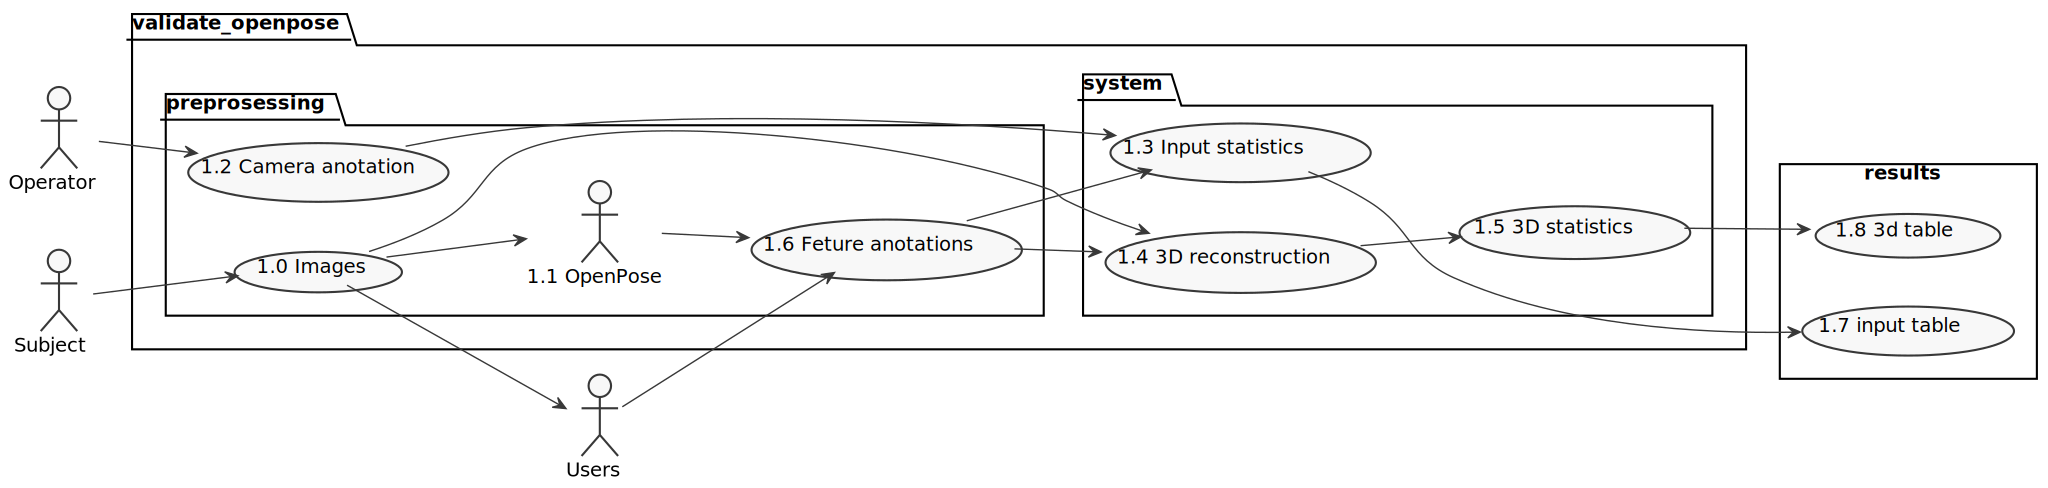
\includegraphics[width=0.9\textwidth]{figures/project_overview.png}
\end{center}
\caption[Project Overview]{In this figure, the overall intended implementation of the system. The subject is the person on the floor while users are the one who annotates the images. The general camera quadrant where the camera was located is annotated by the Operator who took the images. In this image \openpose is displayed as a human, but that is only for clarity that the images are supposed to be annotated equally by both user and \openpose. 1.0 images are stored on the computers file system and can be accessed using Python.}
\label{fig:project_overview}
\end{figure}


\begin{figure}[ht]
\begin{center}
    \includegraphics[width=0.3\textwidth]{figures/feature_anotation.png}
\end{center}
\caption[1.6 feature anotations]{In figure~\ref{fig:project_overview} the block 1.6 Feature Annotations to from \ac{csv} build a database and create an class based API that then 1.3 and 1.4 then uses to future create the validation system. Note that \openpose{ } is only one entity while there are n many users}
\label{fig:1.6.feature_antotation}
\end{figure}



\begin{figure}[ht]
\begin{center}
    \includegraphics[scale=0.4]{figures/openpose_anotation.png}
\end{center}
\caption[1.1 OpenPose anotations]{In this figure the implemented step of 1.1 in figure\ref{fig:project_overview} shows how \openpose takes in images and convert annotate, convert and save the annotations as a CSV file.}
\label{fig:1.1.openpose_anotation}
\end{figure}




\begin{figure}[ht]
\begin{center}
    \includegraphics[scale=0.3]{figures/input_statistics.png}
\end{center}
\caption[1.3 Input statistics]{From block 1.3 in figure~\ref{fig:project_overview}, This figure shows how the input data is processed 1.3.2 loads the annotated data while 1.3.8 and 1.3.9 splits the data up in \openpose and users. 1.3.5 a sample is drawn and the rest of the data makes the 1.3.3 median. 1.3.6 Feature grouping is organising the data according to its features while 1.3.7 organises the data according to Camera quadrant. In 1.3.4 (a,b) the distance equation~\ref{eq:impl:muerror} to calculate the distance from annotated data.}
\label{fig:1.3_input_statistics}
\end{figure}

\begin{figure}[ht]
\begin{center}
    \includegraphics[scale=0.26]{../figures/3D_reconstrution.png}
\end{center}
\caption[1.4 3D reconstruction]{In thins figure the general function for 3D reconstruction is presented. 1.4.1 Load the camera 3D position and how that works is presented in figure\ref{fig:1.4.1_camerapose}. 1.4.2 loads the features for the 2D features on each image. 1.4.3 represents the majority of the human answers while 1.4.4 Is the minority sample. 1.4.5 is the \openpose feature response. 1.4.6 (o,h and s) is the projective geometry deeper explained in figure~\ref{fig:1.4.6.proj_geometry}. 1.4.8 creates a median $\mu$ constructed form the 3D point cloud in 1.4.6.h. 1.4.9 and 1.4.10 Calculates the distance from the median generated in 1.4.8 and the results are sent to the statistics module~\ref{} }
\label{fig:1.4.3D_reconstrution}
\end{figure}

\begin{figure}[ht]
\begin{center}
    \includegraphics[scale=0.3]{../figures/camerapose.png}
\end{center}
\caption[1.4.1 Camera pose]{From figure~\ref{fig:1.4.3D_reconstrution} the position of the camera is calculated in the following steps. 1.4.1.1 Loads the images from the database, 1.4.1.2 Aruco detection detects each individual \aruco in each image and provides the transfer matrix from the camera to the \aruco corner. In 1.4.1.3 the pose quiver connects each corner to each corner in each image figure~\ref{fig:trans_calc} shows the process for that a bit deeper. 1.4.1.4 connect the corner to each corner using the algorithms in~\ref{sub:implement:relative}. 1.4.1.5 Dijkstra is used to derive shortest path from each corner to corner and corner to camera with the position of each step saved in each corner/camera}
\label{fig:1.4.1_camerapose}
\end{figure}


\begin{figure}[ht]
\begin{center}
    \includegraphics[scale=0.35]{../figures/proj_geometry.png}
\end{center}
\caption[1.4.6 Projection geometry]{The projective geometry in figure~\ref{fig:1.4.3D_reconstrution} 1.4.6 (o,h and s) is shown in this figure how first the node projective geometry using the calculations in~\ref{sub:Midpoint} to calculate the projective line out of the camera through a feature from ether \openpose or a human. Shortest distance is the distance between ether two ore more lines for each image and each feature, visually demonstrated in figure~\ref{fig:3Dhuman}. This generates a point cloud with point for each shortest distance.}
\label{fig:1.4.6.proj_geometry}
\end{figure}




Those corners are then identified and connected such that the corner nr 1 in image one is connected to corner nr 1 in image 2.
This process builds a pose quiver of how each corner is connected to each image.
With that process done, the \aruco{ } library can generate the $\vec{t}$ and $\vec{r}$ that determines the camera in relation to that corner.

However, it is not as explained in\ref{sub:implement:relativepath} the path from the \aruco to the camera that is interesting.
Instead, the pose quiver calculates the path from origin to the camera using transfer matrices.
% This is done by using Dijkstra's algorithm for the shortest path and then the algorithm~\ref{alg:inverse},~\ref{alg:relative}
%On the implementation side, this is done by first calculating the path from the origin to the camera using Dijkstra's algorithm.

On the implementation side, the first step in the code is calculating the cumulative transfer matrix from origin to each corner by first setting the origin as $I$.

\input{figures/trans_calc.latex}



% \newpage
\section{Ethics}
\label{sec:ethics}

%I först hand avser vi med ”etik” här forskningsetiska frågor. Innebär ditt val av frågeställning eller metod något forskningsetiskt ställningstagande? Om du till exempel intervjuar personer för ditt arbete, kan du garantera dessa anonymitet och på vilket sätt använder du den information du får av dem? Finns det andra etiska aspekter att beakta i arbetet? Kan det finnas etiska aspekter på resultatet av ditt arbete? Du bör tydligt ange om du anser att ditt arbete inte innehåller några forskningsetiska frågor.

%Du ska också kritiskt granska och analysera ditt arbete med hänsyn till samhälleliga aspekter. Här kan du till exempel diskutera hur ditt arbete förhåller sig till mål som ekonomisk, social och ekologiskt hållbar utveckling. Det kan också finnas juridiska och politiska aspekter på ditt arbete.
According to Starrett, Steve in \cite{starrett2017engineering} the engineer should consider un-ethical use of the implemented system's.
Thus in this part, the system is broken up into previously discussed parts of vision and the robot itself as each faeces different ethical considerations.
As this work uses images of actual humans, the risk is that a picture used in this work is used maliciously.
Other than that, there are no primary ethical considerations for this work.
\newpage
\section{Results}\label{sec:results}

%Här kan du till exempel presentera resultat av experiment, bevis, analys av data etc. Dina resultat måste beskrivas så tydligt att en läsare kan bedöma dem.  Du ska också förklara och analysera resultaten.

The results so far is divided up in two relevant subsections where the first handles the input inference test and the second handles the 3D reconstruction using \aruco corners.
\subsection{OpenPose output inference results}%
\label{sub:res:op_inference}
Using \openpose{ } on a human subject that is located on the ground can provide diverse results dependent on the relative rotation of the body the camera.
How well does it preform when the subject is laying such as in image North in figure~\ref{fig:camera_pos_lables}.
And how is the preference for each label in the \operpose{ } data set against a human labler.

During statistical tests with F/T-test the degrees of freedom will tell you how many data points there is behind the results.
Thus can be shown in table~\ref{tab:results:degfreedom} the degrees of freedom for each label can be found.
While table~\ref{lab:results:human_vs_openpose} shows the degrees of freedom dependent on direction where the camera was located.

From the results in table~\ref{tab:results:human} and table~\ref{lab:results:human_lable} it can be observed that F-test is mostly rejected while the T-test is mostly reported as accept.
This then propose that the $H_0$ hypothesis is weekly rejected as it fails on $\sigma_H = \simgma_O$ but is passed on $\mu_H = \mu_O$.
There fore the $H_1$ hypotheses is accepted and that shows that \openpose{ } do not have same accuracy as an human label setter.



%----------------------------
\begin{table}[htb]
    \begin{center}
    \begin{minipage}{0.4\textwidth}
        \begin{center}
            \input{../results/error_degdf_df.latex}
        \end{center}
        \caption[Degrees of freedom human vs openpose]{The degrees of freedom for human and \openpose is due to the quite limited dataset not in most cases not statistically viable but perhaps it cold work as a marker.}
        \label{tab:results:degfreedom}
    \end{minipage}
    \begin{minipage}{0.4\textwidth}
        \begin{center}
            \input{../results/direction_degdf_df.latex}
        \end{center}
        \caption[Directional degrees of freedom]{The directional degrees of freedom is a bit better because it do not care about the labels, just the total error for that direction. }
        \label{tab:results:dirdegfreedom}
    \end{minipage}
    \end{center}
\end{table}
%----------------------------
\begin{table}[htb]
    \begin{center}
        \input{../results/ftest_pos_df.latex}
    \end{center}
    \caption{The directional results from F-test and T-test}
    \label{lab:results:human_lable}
\end{table}
%----------------------------
\begin{table}[htb]
    \begin{center}
        \input{../results/error_df.latex}
    \end{center}
    \caption[Results in image domain]{The error results for the human vs \openpose in the image domain. Observe the large variance in the forth column that suggests that \openpose have problem finding the correct solution for that label. It can also be observed that the half of the data in comparison with the human is missing from \openpose columns thus indicating again that it could not find a solution to that label.}
    \label{lab:results:human_vs_openpose}
\end{table}
%----------------------------
\begin{table}[htb]
    \begin{center}
        \input{../results/ftest_pds.latex}
    \end{center}
    \caption{Datasets}
    \label{tab:results:human}
\end{table}


\subsection{3D reconstruction using Aruco}%
Reconstruction of the sparce 3D map done by using \aruco{'s} in a pose quiver without solving the bundle adjustment problem was attempted to be solved.
The method derived relied on Dijkstra algorithm and cumulative transfer poses from corner to corner to camera.
An then by solving the epee polar geometry a point cloud is supposed to be generated.
How ever the due to the cumulative output of the algorithms the positions of the camera is never reaching a satisfiable position.



\label{sub:res:3drec}
\begin{figure}
\begin{center}
    \includegraphics[scale=0.6]{results/atlas.png}
\end{center}
\caption[Results from camera mapping]{Reconstructing the camera pose from the images using Dijkstras algorithm  data proved to be a harder problem then initially thought. Ni this results the green numbered nodes seams to find the correct location, but the input camera view nodes in blue do not.}
\label{fig:results:mapreconstruction}
\end{figure}



\newpage
\section{Discussion}
\label{sec:discussion}
% Interpretation of results.
In this report its discussed if \openpose{ } algorithms could be used to derive an accurate position of features to locate a human subject on the floor.
This is done in order with the original questioning if it is accurate enough to do so.


\par In the results~\ref{sec:results} the statistical test is shows that the $H_0$ is rejected due to that the output variance from \openpose{ } is not up to pair with a human.
Thus if a robot attempts to just use \openpose{ } to assist a human there is a chance that the robot misses or in the worst case harms the human subject.
The obvious remedy for that is to not just rely on \openpose{ } but to use external censors and other systems.


\par With the large standard distribution from \openpose{ } in mind, the output from an 3D annotation could only future increase error thus leading to a even less accurate system.
How ever perhaps with sufficient amount of cameras on the scene the median from each camera could be sufficient enough to be used for a grasping procedure.


% Is goal reached? Yes/no why?
\par The goal to reconstruct the point cloud was not reached due to the problem with the last transformation from last corner to to the camera.
The results from that failure can be observed in~\ref{fig:correct_pose} where the positions for the \aruco{ } corners is largely correct while the cameras are not.
Then can the question is can correct position of the camera be derived from just the Dijkstra algorithm or does the bundle adjustment problem need to be solved for correct positions.
As there was no way to measure the absolute position of the camera that question is largely unsolved.
But at least an its an god approximation method that can be used as an base feature to solve the bundle adjustment with in reasonable a time.


% Significance
\par This paper only contains one new data set with just 21 images displayed in Appendices~\ref{sec:appendices} future more the number of annotations of the images are quite low, just six annotations excluding \openpose{ }.
This is also reflected in the results~\ref{sec:results} where the degrees of freedom tables~\ref{tab:results:degfreedom},\ref{lab:results:human_vs_openpose}.


\indent  As shown in Related works~\ref{sec:related_work} there aren't that many other research activity's related to how \openposeS reacts to subjects on the ground.
This work could then with some improvement like a larger dataset can then be used to retrain how \openposeS during such situations.
For the 3D reconstruction part that weren't successful attained the \arucoS, Dijkstra method  cold with a correction to the final camera poses be used to attain sufficient localization to robots and \ac{uav} probably with out solving the bundle adjustment.
On the other way the same method could perhaps be used to make a initial pose quiver to derive an initial position for the bundle adjustment.
The idea could be if a car needs to be retrofitted with cameras that's going to make a 3D approximation of the environment.
The calibration step could just be to throw out a bunch of \arucoS around the car, then taking sufficient amount of pictures with both the cameras in the car and external cameras.
This then with  Dijkstra method with bundle adjustment could derive the camera locations in the set, including the position of the cameras mounted to the car.





%Här presenterar du tolkning av resultaten och bedömer deras signifikans. Diskutera möjliga konsekvenser av resultaten, och presentera eventuella rekommendationer. Det är viktigt att du redogör för om du uppnått de mål du satte upp och därmed besvarat din frågeställning och uppnått syftet med arbetet. Avsnittet ska också innehålla reflektioner kring arbetet, som till exempel dess begränsningar.  Du kan också diskutera lösningar på problem som du identifierat och diskuterat tidigare, eller ta upp andra problem som arbetet inte behandlat, frågor som ej besvarats. Koppla också dina resultat till tidigare arbeten. På så sätt kan diskussionen bli ett samtal med det du skrev i tidigare avsnitt.  Slutligen ska du sätta ditt eget arbete i ett större sammanhang, bredda ditt perspektiv. Kan dina resultatet generaliseras? Kan det du gjort användas i något annat sammanhang?

\newpage
\section{Conclusions}
\label{sec:conclusion}
In this report its attempted to validate \openposeS by comparing it to a human labeller.
The attempted solution is to reconstruct the positions for each label in 3D.
This is done by using a commination of technique's containing \arucoS corners, pose quivering and a Dijkstra method to solve the camera locations.
However the initial result of the output of the \openposS algorithm concludes that the variance is to crude falls the $H_0$ hypotheses, thus the accurate location of a feature could not be attained.
The camera location where also not successfully solved and in any case could probably not be solved completely correctly with out solving the bundle adjustment.

%I detta avsnitt ska du summera rapporten samt presentera slutsatser och slutanalys. Ge en kort översikt av syftet och frågeställningen. Du ska sedan tydligt tala om de viktigaste resultaten, förklara deras signifikans och sätta in dem i sitt sammanhang. Alla slutsatser ska ha stöd i tidigare delar av rapporten.  Du ska däremot inte presentera nya detaljer.

%En expert ska kunna läsa detta avsnitt oberoende av resten av rapporten.


\newpage
%%\input{sections/Acknowledgments}
%% ============================= References ============================
%%% \newpage
\printbibliography
\addcontentsline{toc}{section}{References}

%% ============================ Appendices =============================
\newpage
\begin{appendices}
    \section*{Appendices}
    \label{sec:appendices}
    % \input(sections/99_appendix.tex)
    text

	
\begin{landscape}

\begin{table}[]
    % {\resizebox{10cm}{!}{
        \begin{center}
            \tiny
            \addtolength{\tabcolsep}{-2pt}
        \input{../results/human_error_df.latex}
        \end{center}
    % }}
        \caption{Human error}
    \label{tab:apx:human_error}
\end{table}
\begin{table}[]
    % {\resizebox{10cm}{!}{
        \begin{center}
            \tiny
            \addtolength{\tabcolsep}{-3pt}
        \input{../results/openp_error_df.latex}
        \end{center}
    % }}
        \caption{OpenPose error}
    \label{tab:apx:openp_error}
\end{table}





% % Last on this side
\end{landscape}

	\clearpage
    \input{results/datasets.latex}

	%\input{appendices/appendices2}
	\clearpage
    
\begin{algorithm}
    \caption{Inversing tvec and rvec using Rodrigues transforms}\label{alg:inverse}
    \begin{algorithmic}[1]
        \Procedure{inversePerspective}{rvec, tvec}
        \State $\vec{t} \gets tvec$
        \State $R \gets Rodrigues(rvec)$ \Comment{Vector to matrix}
        \State $R \gets matrix(R)^{T}$ \Comment{Array to transposed matrix}
        \State $\vec{t}^{-1} \gets R \cdot matrix(-\vec{t})$ \Comment{Dot product}
        \State $\vec{r}^{-1} \gets Rodrigues(R)$ \Comment{Rodrigues again}
        \State \textbf{return} $\vec{r}^{-1}, \vec{t}^{-1}$ \Comment{Matrix to vector}
        \EndProcedure
    \end{algorithmic}
\end{algorithm}



\begin{algorithm}
    \begin{algorithmic}[1]
        % \Procedure{relativePosition}{$\vec{t_1}$, $\vec{r_1}$, $\vec{t_2}$, $\vec{r_2}$}
        \Procedure{relativePosition}{rvec1,tvec1,rvec2,tvec2}
       % \Procedure{inversePerspective}{r, t}
        \State $\vec{r_1} \gets reshape(rvec1, (3,1))$ \Comment{Reshape the vectors}
        \State $\vec{t_1} \gets reshape(tvec1, (3,1))$
        \State $\vec{r_2} \gets reshape(rvec2, (3,1))$
        \State $\vec{t_1} \gets reshape(tvec2, (3,1))$
        \State $\vec{r}^{-1}, \vec{t}^{-1} \gets InvercePrespective(\vec{r}, \vec{t})$
             \Comment{Inverse the second marker}
        \State $\text{comp} \gets composeRT(\vec{r_1}, \vec{r_2}, \vec{r}^{-1}, \vec{t}^{-1})$
            \Comment{Creates a composed matrix}
            \State \( \vec{r_{c}},\vec{t_{c}}\gets\text{comp}_{0},\text{comp}_{1}\)
            \Comment{Decompose the matrix}
        \State $\vec{r_{c}} \gets reshape(\vec{r_{c}}, (3,1))$
            \Comment{Reshapes the vectors}
        \State $\vec{t_{c}} \gets reshape(\vec{t_{c}}, (3,1))$
        \State \textbf{return} $\vec{r_{c}},\vec{t_{c}}$
        \EndProcedure
    \end{algorithmic}
    \caption[Relative]{
    Relative position using \textbf{composeRT}, part of \textbf{OpenCV} and the \textbf{invercePrespective} algorithm proposed in Algorithm~\ref{alg:inverse}%
    }
    \label{alg:relative}
\end{algorithm}


\end{appendices}

\end{document}
